\documentclass[29pt,a4paper]{moderncv}

% moderncv themes
%\moderncvtheme[blue]{casual}                 % optional argument are 'blue' (default), 'orange', 'red', 'green', 'grey' and 'roman' (for roman fonts, instead of sans serif fonts)
\moderncvtheme[green]{banking}                % idem

\usepackage[T1]{fontenc}
% character encoding
\usepackage[utf8x]{inputenc}               	% replace by the encoding you are using
\usepackage[italian]{babel}
\usepackage{color}

% adjust the page margins
\usepackage[scale=0.8]{geometry}
\recomputelengths                          	% required when changes are made to page layout lengths

\fancyfoot{} % clear all footer fields
\fancyfoot[L,RO]{\thepage}           		% page number in "outer" position of footer line
\fancyfoot[R,LO]{\footnotesize} 			% other info in 


\begin{document}

\section{\textbf{Change History:}}
\begin{tabbing}
\\\textbf{Date:} ~~~~~~~~~~~~~~~~~\= \textbf{Version Update:}~~~~~~~ \= \textbf{Member:}~~~~~~~~~~~~~~\= \textbf{Description:}\\
2013/08/22 \> 1.0 \> Michelle Peens \> Document created.\\
2013/09/01 \> 1.1 \> Michelle Peens \> Document layout updated.\\
2013/09/10 \> 1.2 \> Michelle Peens \> Database component unit testing added.\\
2013/09/13 \> 1.3 \> Michelle Peens \> Database unit testing updated.\\
2013/09/15 \> 1.4 \> Janine Venter \> Project Scope updated\\
2013/09/15 \> 1.5 \> Janine Venter\> System Description updated\\
2013/09/15 \> 1.6 \> Janine Venter \>Support for Latex and Mimetex updated\\
2013/09/15 \> 1.7 \> Janine Venter \> Messaging updated\\
2013/09/15 \> 1.8 \> Janine Venter \> Main Activity Unit Test\\
2013/09/15 \> 1.9 \> Janine Venter \> Message Adapter Unit Test\\
2013/09/15 \> 2.0 \> Janine Venter \> Open issues added\\
2013/09/15 \> 2.1 \> Janine Venter \> Glossary added\\
2013/09/15 \> 2.2 \> Janine Venter \> Login Test added\\


\end{tabbing}

\newpage
\section{\textbf{Table of Contents:}}
\begin{tabbing}
\\\textbf{Subject}: ~~~~~\= ~~~~~~~~~~~~~~~~~~~~~~~~~~~~~~~~~~~~~~~~~~~~~~~~~~~~~~~~~~~~~~~~~~~~~~~~~~~~~~~~~~~~~~~\= \textbf{Page}:
\\\newline
1. Introduction \> \> 3\\							
\> 1.1 Purpose 	\> 3\\							
\> 1.2 Document Conventions\> 3 					\\
\> 1.3 Project Scope \> 3							\\
\> 1.4 References \> 3							\\
2. System Description \> \> 4					\\
3. Project Testing \> \> 5\\
\> 3.1 Unit Testing \> 5\\
\> 3.2 Integration Testing \>10 \\
\> 3.3 Non Functional Testing \>10 \\
4. Open Issues \> \> 10\\
5. Glossary \> \> 10\\
\end{tabbing}

\newpage
	%\maketitle
	%\vspace{-10mm}
	%Section
	\section*{\textbf{1. Introduction}}
	\vspace{4mm}
	
		\textbf{1.1 Purpose}
			\\The purpose of this document is to explain the scope and results of testing that is performed during the incremental development of the software solution for the Latex Chat Application for our client Mr Will van Heerder.  It will serve as a method for evaluating the progress and correctness of our solution against the set out requirements. Test cases will both include the testing of individual components as they are developed as well as the the testing of the components as one functional unit, after each iteration of our software development process.   \\
		\vspace{1mm}
		
		\noindent \textbf{1.2 Document Conventions}
			\begin{itemize}
				\item Document Formatting: LaTeX
			\end{itemize}
		\vspace{5mm}
		%Section
		
		\noindent \textbf{1.3 Project Scope}
			\\The aim of the project is to develop an open source android XMPP chat client which supports the embedded LaTeX base equations which are rendered as images. LaTeX based equations will be rendered on the handset to produce mathematical equations. Our system will also provide the ability to view, edit and correct equations before sending.
			\parindent 5mm The application will provide a similar functionality to yaxim. Exchange of images and mathematical expressions will be possible through our software solution. The TeXchat application will have the ability to show a preview of the entered text send the equation as LaTeX code and then render it on the receiving end on the client handset.
		\vspace{5mm}
		
	\noindent \textbf{1.4 References}
		\begin{itemize}
		\item Mr. Will van Heerden.
		\end{itemize}
		\vspace{5mm}
		
	%Section
\newpage
	\section*{\textbf{2. System Description}}
	\vspace{4mm}
		\noindent The goal of our software application is to provide a chat service that will allow users to exchange messages and also to send mathematical equations in a rendered image format.  The application is intended to provide a service to users that require the ability and support for a chat client that allows them to communicate more efficiently and effortlessly in a scientific, and mathematical context.  It will provide a more usable mobile version of a Latex chat application.\\ 
		
		\noindent\textbf{Support for LaTeX and MimeTeX Libraries}
		\\The final application will have to make use of a Latex based library for the rendering of equations as images on the mobile device. For this reason we have implemented support for the MimeTeX library, through the use of the Android NDK (Native Development Kit), which allows us to embed the native C/C++ code of the MimeTeX library, in the source code of this release. The library is compiled through Eclipse using a special makefile that sets specific compiler flags to indicate that it is in math mode and not text mode.\\
		
		
		\noindent\textbf{Messaging}
		\\Our final goal is for messaging to be possible between multiple clients, and the support for sending Latex based equations, rendered on the client side and displayed as images on the handheld device. In this release however, our server supports two initial users, and have capabilities for them to send plain text messages and display these in a easy to understand manner.  
		\parindent 5mm The ability to create, render, view and send mathematical equations have been implemented and is currently working. It is now possible to send and receive these equations in image format between the two clients.
		These messages should be stored statically on the device for later retrieval.  For this purpose a SQLite database was implemented.\\
		
		\noindent\textbf{Login}
		\\A user should be authenticated by some type of login component.  This has been implemented during the initial phases of development of this application.  The server that our application uses provides the basic functionality for this authentication component, and uses a username and password based authentication method.
		
\newpage
	\section*{3. Project Testing}
	\noindent \textbf{Unit Testing}\\
	\vspace{4mm}
	\\\textbf{Database Handler Component Unit Test}\\
	The requirements for this component, the database handler, was to set up and successfully create a database and its required tables to persistently save the messages sent to and from clients and keep track of the logged in user. Therefore the unit test for this component includes three cases, namely to set up the database, successfully save information to the database, and to delete chat histories.
	\parindent 5mm Firstly to test if the database and its required tables are in fact successfully created, and not a null value after the create statement is called. The following images depict the results of this unit test on failure of this requirement, i.e the database is null. \\
	
	\begin{figure*}
				\\ \centering
				\\ 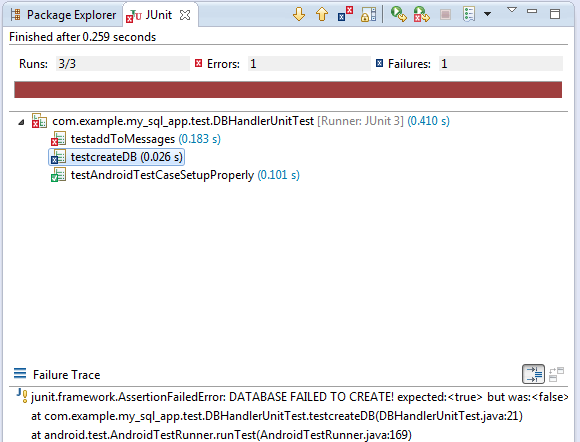
\includegraphics[width=6.0in, height=5.0in]{./databasecreate.png}
				
				\\\caption{[Figure 1] Database Create Test}
	\end{figure*}\\
\newpage	
	Secondly, the next case for this component’s unit test is to ensure that the data, including the messages sent or received, is actually saved to the tables after a method like addToMessages or addRememberMe returns, i.e the data is not found in the database table after the method returned. The images below depict the results of this unit test case on failure of this requirement.\\
	
	\begin{figure*}
				\centering
				\\ 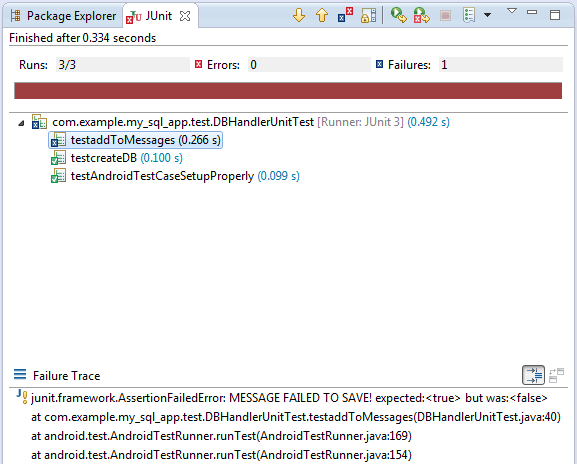
\includegraphics[width=6.0in, height=5.0in]{./messagesave.png}
				\\\caption{[Figure 2] Message Save Unit Test}
	\end{figure*}\\
	
	The third test case is to ensure the when a user wants to delete chat history, all the relevant information is removed from the database. If all the data is successfully deleted, the test case will return true, otherwise it will return false and fail. The image for the failure of this component is depicted below.\\
	
	\begin{figure*}
				\centering
				\\ 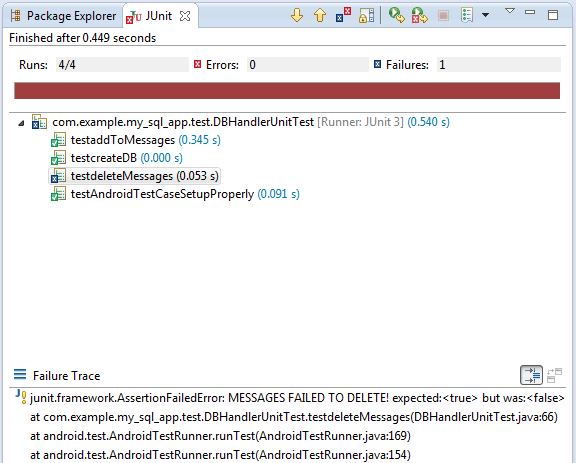
\includegraphics[width=6.0in, height=5.0in]{./deletechat.png}
				\\\caption{[Figure 3] Deleting Message Unit Test}
	\end{figure*}\\
\newpage	
	When these three cases do not fail, and the database and tables are successfully created and the methods addToMessages and addRememberMe successfully saves data, and deleting a chat with a user, removes all the relevant information the following results can be expected from the unit test for this component, i.e when successful.\\
	
	\begin{figure*}
				\centering
				\\ 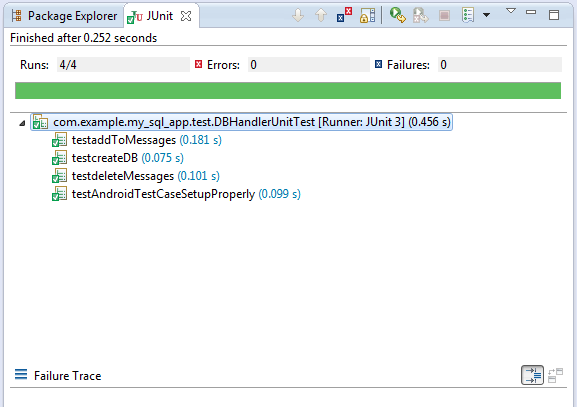
\includegraphics[width=6.0in, height=5.0in]{./success.png}
				\\ \\ \caption{[Figure 4] All Tests Successful}
	\end{figure*}\\
	
\newpage
	\\
	\textbf{Main Activity Unit Test}\\
	\\The Test for Main Activity tests the successful login onto the server.\\
	If the Null test returns null then it means that the test was unsuccessful. Both of those tests are displayed below.
	\\The diagram below depicts the assertNull test which fails when the object returns null.\\
	\\
	\begin{figure*}
					
					\\ 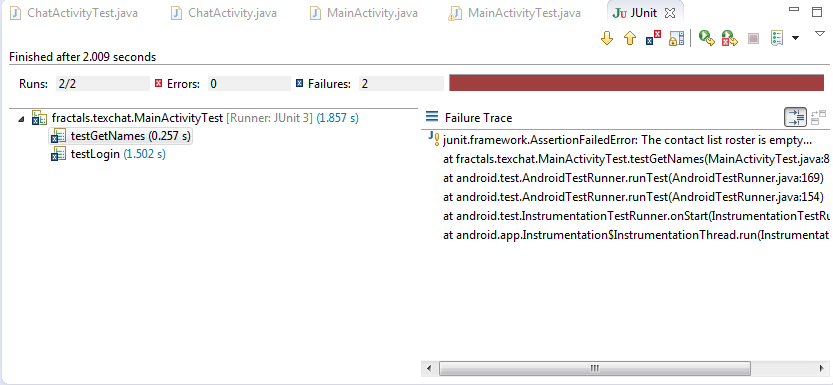
\includegraphics[width=6.0in, height=3.0in]{./loginUnsucc.png}
					\\ \caption{[Figure 5] Logging in to server, Unsuccessful, getting names unsuccessful}
	\end{figure*}\\
	
\newpage	
	\\The diagram below depicts the assertNotNull test which succeeds when the object returns not \\null.\\
	\\
		
	\begin{figure*}
					\\ 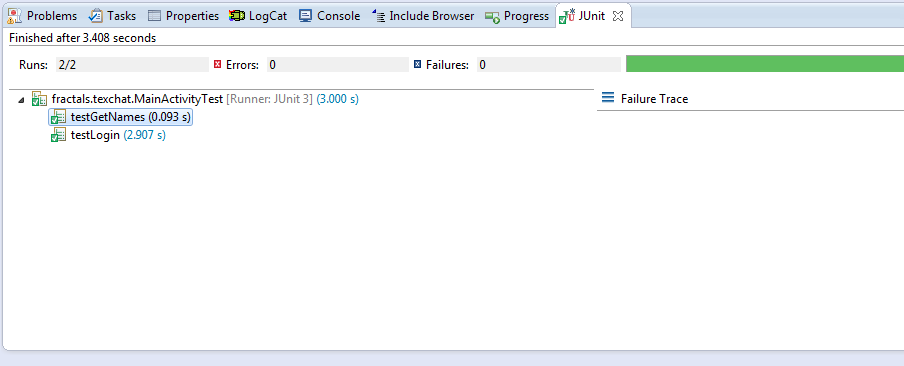
\includegraphics[width=6.0in, height=3.0in]{./loginTestsuccess.png}
					\\\caption{[Figure 6] Logging in to server, Succcessful, get names successful}
	\end{figure*}\\	
	
	\vspace{5mm}
	
	\noindent\textbf{Integration Testing} \\
	Testing complete functionality within the system\\
	
	\noindent\textbf{Non Functional Testing}\\
	Performance testing, load testing\\
	
		\section*{4. Open Issues}	
		\begin{itemize}
			\item Changing the code to adapt to the unit testing.	\\
		\end{itemize} \\

		\section*{5. Glossary}
		\begin{itemize}
			\item Agile - Development methodology
			\item NDK - Native Development Kit
			\item JUnit - Testing Framework
		\end{itemize}
\end{document}